%!TEX root = ../notas_de_clase.tex

%%%%% NOMBRE ESCRIBAS Y FECHA
\renewcommand{\sca}{Matías Azócar}
\renewcommand{\scb}{Carolina Chiu}
\renewcommand{\scc}{Francisco Muñoz}
\renewcommand{\catnum}{2} %numero de catedra
\renewcommand{\fecha}{23 de marzo de 2020}

%%%%%%%%%%%%%%%%%%

% \begin{document}
%Encabezado

% notas al margen
% \ifnum \notasalmargen=1
% \newgeometry{left=1.5cm,top=1.5cm,right=1.5cm, bottom=1.5cm,letterpaper, includeheadfoot, outer=5cm, heightrounded, marginparwidth=4cm, marginparsep=-2.5cm}
% \fi
\NAM{
\newgeometry{left=1.5cm,top=1.5cm,right=1.5cm, bottom=1.5cm,letterpaper, includeheadfoot, outer=5cm, heightrounded, marginparwidth=4cm, marginparsep=-2.5cm}
\savegeometry{notas-al-margen}
}{}

%fin de notas al margen

\fancyhead[L]{Facultad de Ciencias Físicas y Matemáticas}
\fancyhead[R]{Universidad de Chile}
\vspace*{-1.2 cm}
\NAM{\begin{minipage}{0.7\textwidth}}{0.6\textwidth}
\begin{flushleft}
\hspace*{-0.5cm}\textbf{MA4702. Programación Lineal Mixta. 2020.}\\
\hspace*{-0.5cm}\textbf{Profesor:} José Soto\\
\hspace*{-0.5cm}\textbf{Escriba(s):} \sca, \scb ~y \scc.\\
\hspace*{-0.5cm}\textbf{Fecha:} \fecha.
\end{flushleft}
\end{minipage}
\NAM{\begin{minipage}{0.4\textwidth}}{\begin{minipage}{0.36\textwidth}}
\begin{flushright}
\NAM{\hspace*{4.3cm}
\includegraphics[scale=0.15]{fcfm}}{
\includegraphics[scale=0.15]{fcfm}}
\end{flushright}
\end{minipage}
\bigskip

\begin{center}
\LARGE\textbf{Cátedra \catnum}
\end{center}

%Fin encabezado

\section*{Introducción}

En esta cátedra se verán dos temas principales: se comenzará dando un recorrido por la historia de los algoritmos PL/PLM a modo de motivación, para después retomar el contenido de la clase pasada y estudiar más en detalle el concepto de las \textit{formulaciones}.

\section{Historia de Algoritmos PL/PLM}
¿Por qué utilizamos algoritmos de PL/PLM sobre programación no lineal o convexa? Algunas razones son:
\begin{itemize}
    \item Permiten modelar una gran variedad de problemas de la vida real con suficiente generalidad.
    \item Existen buenos algoritmos (a nivel práctico y teórico) y heurísticas\footnote{Una \textbf{heurística} es una técnica diseñada para resolver un problema más rápidamente cuando los métodos clásicos son demasiados lentos, o bien, encontrar una solución cercana al óptimo cuando los métodos clásicos fallan.} que permiten solucionarlas.
    \item Han tenido éxito industrial (existen solvers bien implementados).
\end{itemize}

\subsection*{Orígenes de la Programación Lineal Pura}
\begin{itemize}
    \item \textbf{1827 y 1836}: \textit{Fourier} y \textit{Motzkin} (por separado) describen un método \textbf{finito} para sistemas de desigualdades (conocido como \textit{esquema de eliminación de Fourier-Motzkin}).
    \item \textbf{1937}:\textit{Kantorovich} (Premio Nobel 1975) desarrolla una teoría de dualidad en programación lineal para temas de economía. 
    \item \textbf{1946}: \textit{George Dantzig} desarrolló la base del método Simplex mientras trabajaba para la fuerza aérea de Estados Unidos. Por otro lado, \textit{Jon Von Neumann} desarrolla la teoría de la dualidad en programación lineal.  Ambos junto a Kantorovich se consideran los padres de la programación lineal.
\end{itemize}
%Aquí falta q Simplex no es polinomial y la pregunta de si los PL lo son, etc

\begin{defi}[Algoritmo Polinomial]
Se define como \textit{algoritmo polinomial} a un algoritmo con entrada de $N$ bits, y que ejecuta sus instrucciones en un orden de \Ord[p(N)], donde $p$ es un polinomio. Es decir, un algoritmo con tiempo de ejecución $N^{\Ord[1]}$.
\end{defi}
\begin{defi}[Algoritmo Exponencial]
Se define como \textit{{algoritmo exponencial}} a un algoritmo con entrada de $N$ bits, y que ejecuta sus instrucciones en un orden de \Ord[e^{N}]. Es decir, por ejemplo, un algoritmo al cual le toma $2^{\Ord[N]}$ operaciones en ejecutarse.
\end{defi}
\begin{eje}
Un algoritmo que se tome como máximo $N^{50}$ operaciones en ejecutarse, es un algoritmo polinomial\footnote{Aunque no uno muy eficiente.}.
\end{eje}
\begin{eje}
El algoritmo de Kruskal es polinomial.
\end{eje}
La gran ventaja de este tipo de algoritmos es que si el tamaño de la instancia crece, por ejemplo, se duplica, entonces el tiempo de ejecución sólo se multiplica por una constante. Por ejemplo, un algoritmo con cota $N^k$ en su tiempo de ejecución, al ser alimentado por una instancia de tamaño $2N$, su tiempo cambia a $(2N)^{k}=2^k N^k$.

En cambio, si se está trabajando con un algoritmo exponencial, al duplicar el tamaño de la instancia, la complejidad del algoritmo podría crecer demasiado. Por ejemplo, para un algoritmo con cota $2^{cN}$ en su tiempo de ejecución, la cota para una instancia de tamaño $2N$ se eleva al cuadrado (pues $2^{2cN}=(2^{cN})^2$).

\begin{defi}[Clase P]
La \textit{{clase P}} contiene a aquellos problemas que son solubles en tiempo polinómico.
\end{defi}
\begin{eje}
El problema de calcular un matching es de clase P, pues existe una solución en tiempo polinomial.
\end{eje}

Existe una clase de problemas, llamados NP-completos (cuya definición formal no daremos en este curso) que ocurren muchas veces en la práctica. Se conjetura (no ha sido demostrado) que todos estos problemas no están en P.

\begin{obs}
La pregunta ¿$P=NP$? es aún un problema abierto y es uno de los problemas del milenio\footnote{Es decir, si es que alguien demuestra o refuta la conjetura, ¡se ganará un millón de dolares!.}.
\end{obs}

Se han definido estos conceptos de complejidad para responder a la siguiente pregunta: ¿Qué clase de problema es PL? la pregunta tiene su importancia, pues Klee y Minty (1973) demostraron que Simplex \textbf{no es polinomial}\footnote{Más precisamente, demostraron que hay instancias para los cuales Simplex debe tomar un número superpolinomial de pasos}, a pesar de que es muy rápido en la mayoría de las instancias.

Entonces, ¿Es PL demasiado general como para no estar en P? La respuesta es: ¡No!, en efecto en el año 1979 se demuestra que \textbf{PL está en P}.

\subsection*{Programación Lineal Pura hoy en día}
Ha sido trabajo de los matemáticos el de reducir el tiempo de ejecución del PL. En lo que sigue, $n$ corresponde a variables y $L$ al número de bits que se usan para codificar la entrada.
\begin{itemize}
    \item \textbf{1979}: \textit{Khachiyan} desarrolla el método de la elipsoide para PL (Complejidad $\Ord[n^6L]$).
    \item \textbf{1984}: \textit{Karmakar} desarrolla el método de punto interior (Barrera) para PL (Complejidad $\Ord[n^{3,5}L]$).
    \item \textbf{2015}: \textit{Lee y Sidford} desarrollan la primera mejora en 20 años para flujo en redes (Complejidad $\Ord[n^{2,5}L]$).
    \item \textbf{2019}: \textit{Cohen, Lee y Song} obtienen una complejidad de $\Ord[n^{2,37}L]$ usando multiplicación rápida de matrices.
\end{itemize}

\begin{obs}
Notar que una complejidad de \Ord[n^6 L] es bastante alta, pero al menos es polinomial. Por otro lado, \Ord[n^{2,37} L] ya es una complejidad cercana a una cuadrática, el cuál es un orden más aceptable.
\end{obs}

\begin{obs}
En la práctica, ninguno de estos algoritmos se utiliza (ya que son muy difíciles de implementar, y algunos resultan peores que un algoritmo exponencial en regímenes pequeños). Lo que se usa son mezclas de Simplex, Simplex-dual y Barrera.
\end{obs}

Respondiendo a la pregunta de por qué se prefiere PL/PLM, es porque hoy en día tenemos muchos métodos de resolución a estos problemas. De forma que, se ha avanzado tanto en esta área, que programas lineales que antes tomaban 20 años de procesar, hoy en día se pueden resolver en un segundo. Esto permite utilizar millones de variables y restricciones y resolverlos en un tiempo prudente.

\subsection*{¿Qué pasa con PLE y PLM?}
\begin{itemize}
    \item En la década de 1960 sale el primer solver comercial.
    \item Las siguientes décadas se dedican a crear mejoras en la implementación de PL.
    \item En la década de 1990 aparecen solvers nuevos, como \textit{CPLEX} (ILOG), \textit{MINTO} (Gerogia Tech) y \textit{XpressMP} (comercial).
    \item En el año 2007 IBM compra ILOG.
    \item Los creadores originales de \textit{CPLEX} no se involucran con IBM, y en su lugar fundan \textit{Gurobi} en el año 2009.
\end{itemize}

Hoy en día, los problemas de programación lineal entera se pueden resolver de forma rápida debido a que se han incorporado una serie de ideas (que se verán más adelante en el curso) a los solvers previamente mencionados. Algunas de ellas son:
\begin{itemize}
    \item Aproximación sucesiva de PLE por PL.
    \item Agregar planos cortantes, es decir, incluir restricciones sin perder puntos factibles (mejora en la formulación).
    \item \textit{Branch and Bound}: es la base de los algoritmos PLE. La idea es que si hay un conjunto finito de puntos que pueden ser solución, se pueden enumerar de manera sistemática (como árbol) y es posible darse cuenta que hay ramas del árbol que no pueden ser solución.
    \item Planos cortantes genéricos: cortes que se generan automáticamente (Gomory, MIR, etc.)
    \item Presolver (Técnicas de reducción de tamaño).
    \item Generación de filas y columnas; Simetría; Heurísticas; entre otras.
\end{itemize}

Probablemente PLE no está en P (se puede probar que es NP-Completo). Sin embargo, los solvers disponibles actualmente son capaces de:
\begin{itemize}
    \item Realizar buenas aproximaciones de soluciones de PLE con millones de variables y restricciones. Estas soluciones son factibles y pueden reportar que se encuentran cerca del óptimo. (para hacer esto, no se necesita que el usuario sea un experto, sólo basta con saber ocupar dichos solvers).
    \item Resolver a optimalidad muchas clases de subproblemas.
    \item Todo eso se hace prácticamente sin intervención del usuario.
\end{itemize}

\section{Formulaciones}
\begin{defi}[Poliedro] Un \emph{poliedro} $P$ es un conjunto lineal puro, es decir
$$P=P(A,b)=\{x\in \RR^n:Ax\leq b\}$$
con $A\subseteq \RR^{n\times m}$ y $b\in \RR^n$
\end{defi}
\begin{itemize}
    \item Si $A$ y $b$ pueden ser escogidos racionales (es decir, sus componentes pueden ser escogidas racionales): $P$ es un \textbf{poliedro racional}.
    \item Si $P$ es acortado: se llama \textbf{polítopo}.
\end{itemize}
\begin{obs}
Dado que los poliedros son intersecciones finitas de semiplanos, y los semiplanos son conjuntos convexos, entonces los poliedros son \textit{conjuntos convexos}.
\end{obs}
\begin{defi}[Formulación] Un poliedro $P$ es una \emph{formulación} para un conjunto $S\subseteq\ZZ^E \times \RR^ C$ si:
$$S=P\cap (\ZZ^E \times \RR^C)$$
\end{defi}
En otras palabras, una formulación es un poliedro que aproxima externamente bien a algún conjunto.

\begin{eje} \label{eje:formulacion1}
En la Figura \ref{fig:formulacion1}, se puede observar un poliedro $P$ (conjunto verde) que es una formulación de un conjunto $S$ (puntos rojos), pues $$S = P \cap \ZZ^{E}$$ 
\begin{figure}[H] 
    \centering
    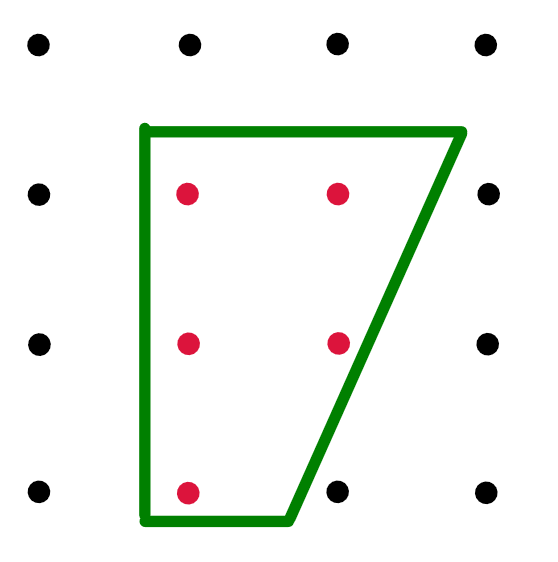
\includegraphics[scale=0.3]{formulacion1.png}
    \caption{Primer ejemplo de una formulación.}
    \label{fig:formulacion1}
\end{figure}
\end{eje}

Podemos notar que las formulaciones no son necesariamente únicas, en efecto, en el Ejemplo \ref{eje:formulacion1} se puede encontrar otro poliedro $P'$, tal como se presenta en el siguiente ejemplo:

\begin{eje} \label{eje:formulacion2}
En la imagen \ref{fig:formulacion2}, se puede observar un poliedro $P'$ (conjunto azul) que es una formulación de un conjunto $S$ (puntos rojos), pues $$S = P' \cap \ZZ^{E}$$ 
\begin{figure}[H] 
    \centering
    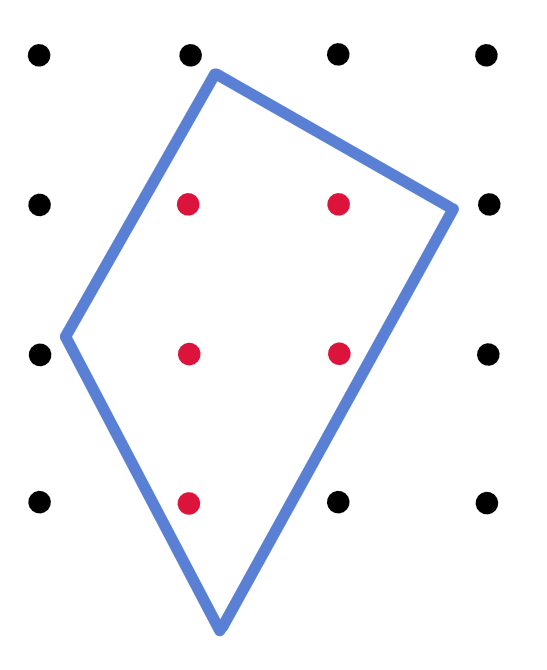
\includegraphics[scale=0.3]{formulacion2.png}
    \caption{Segundo ejemplo de una formulación.}
    \label{fig:formulacion2}
\end{figure}
\end{eje}

Dicho esto, nos podemos preguntar: ¿Cuál de todas las formulaciones ocupar? La respuesta que nace naturalmente es: ocupar la formulación minimal para $S$. Esto se puede lograr ocupando como formulación para $S$ su envoltura convexa, vale decir, $\conv S$. Una representación de lo anteriormente dicho se puede observar en la siguiente figura:

\begin{figure}[H] 
    \centering
    
\includegraphics[scale=0.3]{formulacion3.png}
    \caption{Formulación minimal para $S$: su envoltura convexa.}
    \label{fig:formulacion3}
\end{figure}


Formalizando lo comentado anteriormente en los ejemplos, $P$ es buena formulación de $S$ si es que lo \emph{aproxima} apropiadamente. Para empezar, al menos, sabemos que debemos tener lo siguiente 
\begin{center}
$S\subseteq P$
\end{center}
\begin{itemize}

    \item Sean $P_1\subseteq P_2$ dos formulaciones para el mismo conjunto. En este contexto, diremos que $P_1$ es \emph{mejor} que $P_2$.
    
    Posterior a esto, no es difícil pensar que el mejor de todos los casos será tomar como formulación la envoltura convexa (esto puede, y debería, ser demostrado). Justamente por eso tenemos lo siguiente
    
    \item Si $P=\conv(S)$ entonces $P$ es \emph{formulación ideal} de $S$.
\end{itemize}

\begin{obs}No todos los conjuntos lineales mixtos admiten formulaciones ideales. \end{obs}

En la siguiente figura se puede apreciar un ejemplo de lo anterior, pues, para la primera restricción (gráficamente, la diagonal) no hay valores que se alcancen en la frontera. Esto, pues habría que solucionar $-\sqrt2 x+y=0$ con $x,\ y$ enteros. Sin embargo, por la irracionalidad de $\sqrt2$ no habrá un punto $(x,y)$ que resuelva tal ecuación. Lo que sucederá es que iremos tomando una cantidad infinita de puntos que se acerquen, pero eso no define un poliedro. Así, se evidencia que hay conjuntos que no admiten formulación ideal. 
\begin{figure}[H]
    \centering
    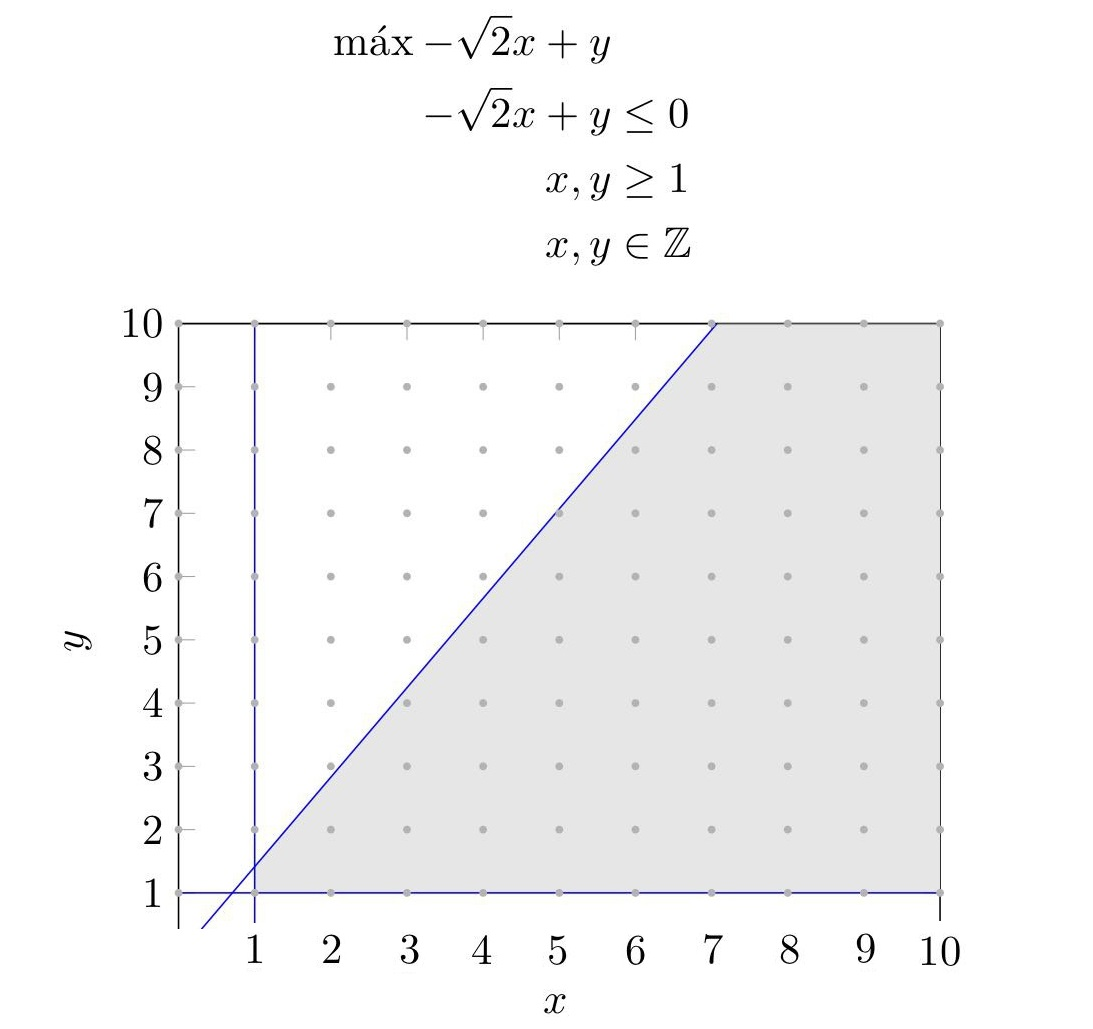
\includegraphics[scale=0.18]{Imagen1.jpg}
    \caption{Ejemplo de PLM donde no existe formulación ideal.}
    \label{fig:NoExistenceIdeal}
\end{figure}

Notemos que lo anterior no sucede para un PL puro, recordando del curso de optimización, que todo PL factible y con objetivo acotado alcanza su óptimo.

\begin{teo}
Sea (\textit{M}) un PLM con datos racionales. Si su relajación lineal (\textit{P}) es acotado en la dirección de optimización, entonces o bien (\textit{M}) tiene óptimo finito racional y alcanzable, o bien (\textit{M}) es infactible.
\end{teo}

\begin{eje}[Uncapacitated Facility Location] Un problema clásico en Investigación de Operaciones es el de \emph{Uncapacitated Facility Location}. Definimos ahora lo que se recibe como información y lo que busca hallar el problema.

\begin{figure}[H]
    \centering
    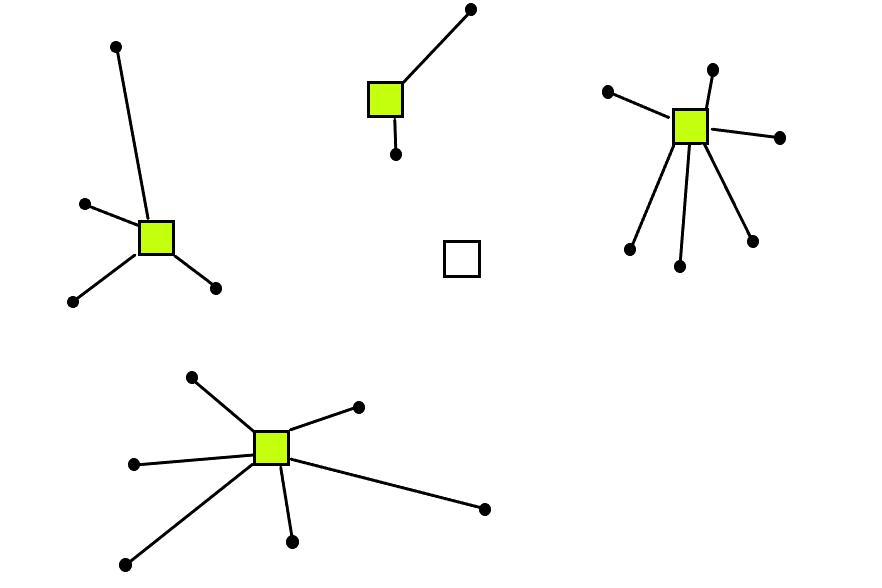
\includegraphics[scale=0.25]{UFL.png}
    \caption{Visualización del problema \textit{Uncapacitated Facility Location}.}
    \label{fig:UFL}
\end{figure}

\textbf{Entrada:} $n$ clientes y $m$ ubicaciones de bodegas. Existe un costo fijo $c_j\geq 0,\ \forall j\in [m]$ asociado a la apertura de una bodega y un costo de conexión $d_{ij}\geq 0$ por conectar a un cliente $i$ con una bodega $j$, $\forall i\in[n]$, $\forall j\in[m]$.

\textbf{Objetivo:} Abrir bodegas y conectar clientes a bodegas abiertas incurriendo en un costo total mínimo.

Construiremos una formulación para el problema:

Para ello haremos uso de dos variables binarias:
$$y_j=\begin{cases}1\text{ si la bodega }j\text{ abre.}\\
0\text{ si no lo hace}\end{cases}\hspace{0.5cm}x_{ij}=\begin{cases}1\text{ si el cliente } i\text{ conecta con la bodega }j\\
0\text{ si no lo hace}
\end{cases}$$
De esta forma, procederemos a plantear la formulación. Queremos minimizar el costo total, así, el objetivo será:
$$\text{(FL1)}\hspace{0.5cm}\min \sum_{j\in[m]}c_j y_j + \sum_{i\in [n]}\sum_{j\in[m]}x_{ij}d_{ij}$$
El primer término será el asociado a los costos fijos de las bodegas y el de la derecha el costo de conexión cliente-bodega total.

Ahora, las restricciones serán las siguientes:

\begin{equation*}
    \begin{array}{rll}
        s.a.&\sum\limits_{j\in[m]}x_{ij}=1&\forall i \in [n]\\
        &\sum\limits_{i\in [n]}x_{ij}\leq n\cdot y_j&\forall j \in [m]\\
        &x_{ij},\ y_{j}\in\{0,1\}&\forall i\in[n]\text{ }\forall j\in[m]
    \end{array}
\end{equation*}

La primera restricción es la que indica que de todas las bodegas, el cliente \emph{debe} estar asociado a una. (Podría ser reemplazado por la restricción de estar asociado al menos con una). La segunda viene de la siguiente situación:
\begin{itemize}
    \item Si la bodega no abre ($y_j=0$) no pueden haber clientes asociados a esa bodega, luego, como los $x_{ij}$ son no negativos, deben ser todos cero.
    \item Si la bodega abre ($y_j=1$) entonces pueden haber como máximo $n$ clientes asociados a esa bodega (pues ese es el número total de clientes)
\end{itemize}
La tercera restricción viene del hecho de que definimos $x_{ij}$ y $y_j$ como variables binarias. 

El objetivo junto a las tres restricciones definen la formulación que hemos construido.
\end{eje}


\begin{eje}[Problema de Asignación] Un problema al que probablemente usted ha podido enfrentarse en Algoritmos Combinatoriales es el \emph{problema de asignación.}

\begin{figure}[thb]
\centering
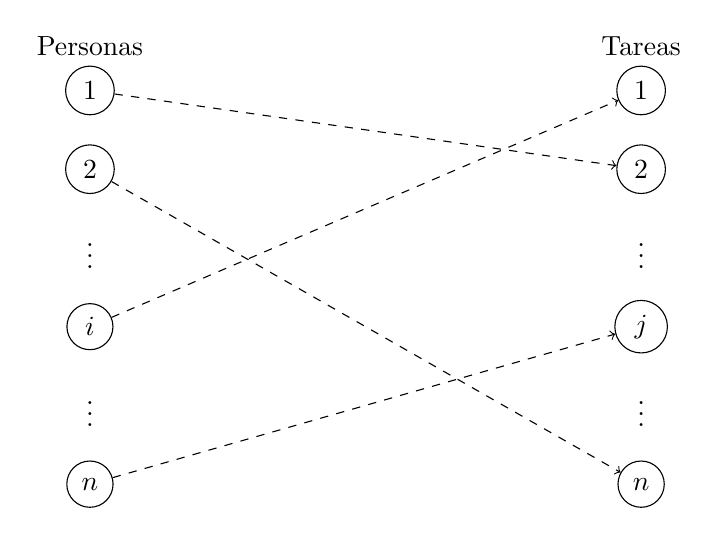
\begin{tikzpicture}[scale=1]
    %Origen
    \node[draw,circle] (p1) [label=above:Personas]   at (0,5) {1};
    \node[draw,circle] (p2) []                       at (0,4) {2};
    \node              ()                                            at (0,3) {$\vdots$};
    \node[draw,circle] (pi) []                       at (0,2) {$i$};
    \node              ()                                            at (0,1) {$\vdots$};
    \node[draw,circle] (pn) []                       at (0,0) {$n$};
    %Destino
    \node[draw,circle] (t1) [label=above:Tareas] at (7,5) {1};
    \node[draw,circle] (t2) []                      at (7,4) {2};
    \node              ()                                            at (7,3) {$\vdots$};
    \node[draw,circle] (tj) []                      at (7,2) {$j$};
    \node              ()                                            at (7,1) {$\vdots$};
    \node[draw,circle] (tn) []                      at (7,0) {$n$};
    \draw[->, dashed] (p1) -- (t2);
    \draw[->, dashed] (p2) -- (tn);
    \draw[->, dashed] (pi) -- (t1);
    \draw[->, dashed] (pn) -- (tj);    
\end{tikzpicture}
\caption{Problema de Asignacion.}
\label{fig:prob_asign}
\end{figure}

\textbf{Entrada:} $n$ tareas y $n$ personas. Cada persona debe realizar \emph{exactamente} una tarea. $c_{ij}$ es el costo incurrido por la persona $i$ al realizar la tarea $j$.

\textbf{Objetivo:} Encontrar la asignación de costo total mínimo.



Construiremos una formulación para el problema:

Para ello haremos uso de una variables binaria:
$$x_{ij}=\begin{cases}1\text{ si la persona } i\text{ realiza la tarea }j\\
0\text{ si no lo hace}
\end{cases}$$
Así, procedemos. Queremos minimizar el costo total, así, el objetivo será:
$$\text{(}A\text{)}\hspace{0.5cm} \min \sum_{i\in[n]}\sum_{j\in [n]}c_{ij} x_{ij}$$
El término proviene de sumar los costos de las personas (suma sobre $i$) asociadas a las tareas (suma sobre $j$), los cuales contaremos solo si la persona $i$ realiza la tarea $j$.

Ahora, las restricciones serán las siguientes:

\begin{equation*}
    \begin{array}{rll}
        s.a.&\sum\limits_{j\in[n]}x_{ij}=1&\forall i \in [n]\\
        &\sum\limits_{i\in [n]}x_{ij}=1&\forall j \in [n]\\
        &x_{ij},\in\{0,1\}&\forall i\in[n]\text{ }\forall j\in[n]
    \end{array}
\end{equation*}
El objetivo junto a las tres restricciones definen la formulación que hemos construido. \\

Ahora, definiremos lo siguiente:
\begin{itemize}
    \item $S$: Dominio de ($A$)
    \item $D$: Relajación de ($A$)
\end{itemize}


Gracias a un importante resultado de Birkhoff y Von Neumann sabemos que todo punto en $P$ es combinación convexa de puntos enteros (en $S$), Luego, $P$ es ideal.
\end{eje}

Para finalizar la clase, se presenta un caso interesante. \\
Sea ($M$) un PLE (totalmente) acotado, con dominio $S$. Luego $S$ es finito. ¿Tiene formulación ideal?
\begin{align*}
    S &=\{s_i\}_{i=1}^K\\
    \conv(S) &=\{x=\sum_{i=1}^K \lambda_i s_i:\lambda_i\geq 0,\ \sum_{i=1}^K \lambda_i=1\}
\end{align*}
Surge así la pregunta\ldots
¿La envoltura convexa de un conjunto finito de puntos es un poliedro? (esto puede ser respondido a través del estudio de teoría poliedral).


\begin{comment}
En la red hay bastante material para aprender a usar esta herramienta. Como ejemplo, les recomiendo visitar
\url{http://latex-project.org/guides/} y \url{http://texblog.net/}.

Además, es bueno empezar a seguir buenas prácticas, dejando de lado un montón de comandos que están obsoletos (en particular, reemplazar \verb+\eqnarray+ y \verb+$$ ... $$+ por los más modernos \verb+\align+ y \verb+\[ ... \]+).

\subsection{Recomendaciones para escribir un apunte}
Es bueno comenzar cada clase con una frase introductoria, explicando lo que se va a ver. No llegue y copie textualmente lo que se ve en la pizarra / video sin incorporar comentarios que aclaren (en clases, suelo decir mucho más de lo que escribo).

Recuerde que las ecuaciones también son parte del texto, y luego deben cumplir las reglas de puntuación (por ejemplo, usar comas y puntos
finales).

\subsection{Algunos ejemplos}

\subsubsection*{Uso simple de macros:}
\begin{defi}[Cintura de un grafo]
 La \emph{cintura} de un grafo es el largo del ciclo más corto. Si el grafo es acíclico, se define como $+\infty$.
Denotaremos la cintura de $G$ por $\cin(G)\in \ZZ$. 
\end{defi}
Observar (en la fuente) la definici\'on de las macros \verb+\Z+ y \verb+\cin+.

\begin{lem}
 Si $G$ es un grafo bipartito entonces $\cin(G)\ge 3$.
\end{lem}

M\'as ejemplos: Escriba $\min(X)$ (\begin{verb}$\min(X)$\end{verb}) en vez de $min(X)$ (el \'ultimo parece producto de $m$, $i$ y $n$). 
Por lo mismo, escriba tambi\'en $X_{\text{opt}}$ (\begin{verb}$X_{\text{opt}}$\end{verb}) en vez de $X_{opt}$.


\subsubsection*{Ecuaciones alineadas.}

No es difícil escribir ecuaciones que tengan una sola alineación como
\begin{align}
\psi(n)
&= \frac{(2n)!}{n! 2^n} = \frac{(2n)(2n-1) \dotsm (n+1)}{2^n} \notag \\
&\geq \left( \frac{n}{2} \right)^n. \label{eqn:interesante}
\end{align}

Sin embargo, escribir un PL en \LaTeX{} puede ser complicado. Un formato tipo para escribir simultáneamente un primal y un dual es el siguiente:

\begin{alignat*}{5}
&\max\        & \sum_{ij \in E} x_{ij}w_{ij} &		 &                      &\qquad\qquad \min\        &\sum_{i \in V}y_i&\\
&\text{s.a. } & \sum_{j\colon j\neq i} x_{ij}&\leq 1 &\quad\forall i \in V  &\qquad\qquad \text{s.a. } &y_i+y_j &\geq w_{ij} &\quad\forall ij \in E\\
&	          & x_{ij}                       &\geq 0 &\quad\forall ij \in E &\qquad\quad               &y_i &\geq 0      &\quad\forall i \in V.
\end{alignat*}

\medskip
Este es solo un documento de ejemplo. Entre otras cosas \LaTeX{} permite escribir fácilmente
\begin{itemize}
  \item Matrices.
  \item Integrales.
  \item Tablas.
  \item Listas.
  \item etc.
\end{itemize}
 
\subsection{Ejemplo}

Como ejemplo adjunto el principio de la primera cátedra a continuación.

\begin{defi}[Problema de optimización e instancias] Un \textit{problema de optimización} $\mathcal{P}$ es un conjunto de \textit{instancias}. Cada \textit{instancia} está definida por:
\begin{itemize}
\item Un conjunto factible $S$.
\item Una función a optimizar $f: S \to \RR$.
\item Un objetivo, minimizar o maximizar la función $f$ en dicho conjunto $S$.
\end{itemize}
\end{defi}

Usualmente las instancias se describen de manera implícita o compacta.  Por ejemplo:

\begin{eje}[Árbol cubridor de peso mínimo -- minimum spanning tree, MST]
Cada instancia del problema (MST) se describe de manera compacta indicando un grafo $G=(V,E)$ con pesos en las aristas $w\colon E \to \RR_+$. De estos datos uno puede deducir el conjunto $S$ de todos los árboles cubridores de $G$, y para cada árbol $T\in \mathcal{S}$, el valor de la función es la suma de los pesos de las aristas $w(T)=\sum_{e\in T}w(e)$. El objetivo es minimizar la función de peso $w$.
\end{eje}
\end{comment}
%%NO ESTA LISTO TENGO Q TERMINAR EL ULTIMO EJEMPLO UWU

% \end{document}

%%%%%%%%%%%%%%%%%%%%%%%%%%%%%%%%%%%%%%%%%%%%%%%%%%%%%%%%%%%%%%%%%%%%%%%%%%%%%%%%%%%%%%%%%%%%
%%%%%%%%%%%%%%%%%%%%%%%%%%%%%%%%%%%%%%%%%%%%%%%%%%%%%%%%%%%%%%%%%%%%%%%%%%%%%%%%%%%%%%%%%%%%

